% Options for packages loaded elsewhere
\PassOptionsToPackage{unicode}{hyperref}
\PassOptionsToPackage{hyphens}{url}
\PassOptionsToPackage{dvipsnames,svgnames*,x11names*}{xcolor}
%
\documentclass[
  12pt,
  pagebackref]{article}
\usepackage{lmodern}
\usepackage{amssymb,amsmath}
\usepackage{ifxetex,ifluatex}
\ifnum 0\ifxetex 1\fi\ifluatex 1\fi=0 % if pdftex
  \usepackage[T1]{fontenc}
  \usepackage[utf8]{inputenc}
  \usepackage{textcomp} % provide euro and other symbols
\else % if luatex or xetex
  \usepackage{unicode-math}
  \defaultfontfeatures{Scale=MatchLowercase}
  \defaultfontfeatures[\rmfamily]{Ligatures=TeX,Scale=1}
\fi
% Use upquote if available, for straight quotes in verbatim environments
\IfFileExists{upquote.sty}{\usepackage{upquote}}{}
\IfFileExists{microtype.sty}{% use microtype if available
  \usepackage[]{microtype}
  \UseMicrotypeSet[protrusion]{basicmath} % disable protrusion for tt fonts
}{}
\makeatletter
\@ifundefined{KOMAClassName}{% if non-KOMA class
  \IfFileExists{parskip.sty}{%
    \usepackage{parskip}
  }{% else
    \setlength{\parindent}{0pt}
    \setlength{\parskip}{6pt plus 2pt minus 1pt}}
}{% if KOMA class
  \KOMAoptions{parskip=half}}
\makeatother
\usepackage{xcolor}
\IfFileExists{xurl.sty}{\usepackage{xurl}}{} % add URL line breaks if available
\IfFileExists{bookmark.sty}{\usepackage{bookmark}}{\usepackage{hyperref}}
\hypersetup{
  pdfauthor={Dmitry Sorokin},
  colorlinks=true,
  linkcolor=mypink,
  filecolor=myblue,
  citecolor=mypink,
  urlcolor=mypink,
  pdfcreator={LaTeX via pandoc}}
\urlstyle{same} % disable monospaced font for URLs
\usepackage[margin=1in]{geometry}
\usepackage{graphicx}
\makeatletter
\def\maxwidth{\ifdim\Gin@nat@width>\linewidth\linewidth\else\Gin@nat@width\fi}
\def\maxheight{\ifdim\Gin@nat@height>\textheight\textheight\else\Gin@nat@height\fi}
\makeatother
% Scale images if necessary, so that they will not overflow the page
% margins by default, and it is still possible to overwrite the defaults
% using explicit options in \includegraphics[width, height, ...]{}
\setkeys{Gin}{width=\maxwidth,height=\maxheight,keepaspectratio}
% Set default figure placement to htbp
\makeatletter
\def\fps@figure{htbp}
\makeatother
\setlength{\emergencystretch}{3em} % prevent overfull lines
\providecommand{\tightlist}{%
  \setlength{\itemsep}{0pt}\setlength{\parskip}{0pt}}
\setcounter{secnumdepth}{5}
\renewcommand{\ttdefault}{cmr} % change the font of inline R results to normal
\renewcommand*{\backref}[1]{}
\renewcommand*{\backrefalt}[4]{%
    \ifcase #1 (Not cited.)%
    \or        [Cited on page~#2.]%
    \else      [Cited on pages~#2.]%
    \fi}
\setlength{\parindent}{25pt}
\setlength{\parskip}{0pt}
\setlength{\skip\footins}{0.25cm} % margin before footnotes
\definecolor{myblue}{RGB}{31, 61, 122}
\definecolor{mypink}{RGB}{204, 0, 82}
\newtheorem{assumption}{Assumption}[section]
\newtheorem{proposition}{Proposition}[section]
\newcommand{\EE}[1]{\mathbb{E}\left[#1\right]}
\newcommand{\PP}[1]{\mathbb{P}\left(#1\right)}
\newcommand{\CP}[2]{\mathbb{P}\left(#1 \,| \, #2 \right)}
\newcommand{\CE}[2]{\mathbb{E}\left[#1\,|\,#2 \right]}
\usepackage[bottom]{footmisc}
\usepackage[doublespacing]{setspace}
\usepackage[tableposition=top]{caption}
\usepackage{dsfont}
\usepackage{booktabs}
\usepackage{makecell}
\usepackage[]{natbib}
\bibliographystyle{plainnat}

\title{Consumer Reviews and Product Discounts:\\
Evidence From Video Games}
\author{Dmitry Sorokin}
\date{\texttt{r\ format(Sys.time(),\ \textquotesingle{}\%B\ \%d,\ \%Y\textquotesingle{})}}

\begin{document}
\maketitle

\hypertarget{introduction}{%
\section{Introduction}\label{introduction}}

\hypertarget{literature-review}{%
\section{Literature Review}\label{literature-review}}

This paper contributes to several closely related literatures in
economics and marketing. The oldest of these is the literature
investigating the impact of online consumer reviews on sales. An
extensive review of the studies focusing on this topic and their
meta-analysis is provided, for example, by \citet{Floyd14}. In a seminal
contribution in this literature, \citet{ChevalierMayzlin06} uses a
difference-in-differences approach, exploiting the differences in
reviews for the same books across Amazon.com and Barnesandnoble.com, to
argue that better reviews causally improve sales. A similar approach
applied to the same market was recently used by
\citet{ReimersWaldfogel20}, who reaffirm the importance of reviews for
sales of books and quantify the welfare implications of the
informational content of consumer reviews. \citet{ZhuZhang10} exploit
differences between two different video games consoles rather than
websites, and find that review ratings matter only for less popular
games.

For identification, the difference-in-differences approach relies on the
existence of several comparable platforms, and assumes that the
unobserved platform-specific tastes for those platforms are fixed.
Another approach to identification exploits the rounding of the review
data that platforms use to produce simple visual review labels. For
example, Yelp.com, a popular restaurant comparison service, assigns 4
stars to restaurants that have an average review score between 4 and
4.24 (out of 5), but 4.5 stars to restaurants with an average score
between 4.25 and 4.74. \citet{AndersonMagruder12} and \citet{Luca16}
develop a regression discontinuity approach exploiting this rounding to
show that an additional half-star on Yelp.com increases restaurants'
traffic and revenue. \citet{SorokinStevens20} applies a similar approach
to the video games market and also finds that better review labels
increase sales, albeit raising some concerns about the validity of the
approach. In the absence of direct sales data, \citet{SorokinStevens20}
uses a particular regression specification that extracts the information
on sales from the video games' usage data. The present paper supplements
the panel methods in \citet{SorokinStevens20} by offering a structural
way to estimate the effect of reviews on sales in the absence of direct
sales data.

With benefits of having good reviews come the incentives to influence
the reviews in order to reap those benefits. There are several ways
firms can affect their online reviews. One is review fraud.
\citet{Mayzlin14} provides evidence that small hotel owners leave
negative reviews for their competitors, and good reviews for themselves.
\citet{LucaZervas16} provide similar evidence for restaurants on Yelp. A
more honest way for a firm to influence reviews is by assuming an active
approach to review management, and to publicly respond to reviews
published online. \citet{GuYe14} provide evidence that consumers who had
left a negative review about their hotel experience in the past were
more likely to leave a positive review of the same hotel after a future
stay if their previous review was responded to by the management.
\citet{XieEtAl17} shows that lengthy in-depth managerial responses to
negative reviews are associated with better financial performance in the
future. This literature has also been concerned with how consumers
change their reviewing behavior when managers start responding to
reviews, essentially moving from studying individual responses to
describing equilibrium outcomes. In somewhat contradictory findings,
\citet{ProserpioZervas17} argues that hotels responding to bad reviews
experience an increase in both the valence and the volume of their
reviews, attributing it to consumers' reluctance to leave short
indefensible reviews in a situation when they can be responded to, while
\citet{ChevalierEtAl18} finds the opposite effect in the same market,
arguing that managerial responses encourage negative review activity,
because consumers get a signal that the firm is ``listening'' to them,
and are then stimulated to leave negative reviews that they deem more
influential.

Direct ways of managing online reputation discussed above, however, are
not the only avenues through which businesses can affect their reviews.
Reviews are left by customers, and the happier they are, the better
reviews they should leave, at least in principle. Another strand of
literature is studying whether different kinds of promotions have an
effect on firms' online reputation. In a seminal study,
\citet{ByersEtAl12} documents that restaurants receive substantially
worse reviews after running a Groupon price promotion. They present
evidence that customers attracted by the promotion are different from
regular customers, and that they are more likely to be trying out a new
restaurant or cuisine while using the Groupon voucher, which can explain
the reasons behind their dissatisfaction. Thus, the paper cautions
against running price promotions in an attempt to poach new customers
and improve the online reputation. \citet{Li16} confirms the finding in
the same setting, but finds that restaurants with fewer and worse
reviews can actually benefit from participating in a Groupon promotion.
\citet{ZhuEtAl19} shows that customers who received a discount leave
more positive, albeit less informative, reviews. In an experimental
study on Ebay, \citet{CabralLi15} also find that offering a rebate for
leaving (any) review significantly decreased the likelihood of negative
feedback, and they provide evidence that this is due to reciprocity on
the side of the clients, rather than the differences between customers
buying with a rebate and without it.

The present study contributes to this literature by providing novel
evidence from a new market. I show that customers buying computer games
are significantly more likely to leave positive reviews during
discounts. More importantly, I go beyond the descriptive nature of the
other papers in the literature, and show that firms leverage this fact
to improve their reviews by giving discounts, thus providing evidence of
a novel reputation management behavior. A study similar in spirit to
mine is that of \citet{Zegners17}, who argues that less-known authors of
eBooks on a crowded online marketplace are more likely to give their
books out for free in order to build reputation and escape the ``zero
reviews trap''. However, this study also finds that books are more
likely to solicit negative feedback when sold for free, which somewhat
undermines the strategy. Similar to \citet{ByersEtAl12},
\citet{Zegners17} argues that purchasers of free books differ from the
purchasers of regular books in their observable characteristics, and
explains the negativity of the reviews by the selection effect.

\hypertarget{institutional-setting-and-data}{%
\section{Institutional Setting and
Data}\label{institutional-setting-and-data}}

\hypertarget{steam-marketplace}{%
\subsection{Steam Marketplace}\label{steam-marketplace}}

Steam is arguably the largest online marketplace for selling computer
games in the world. Founded in 2003, in 2013 it was responsible for
about 75\% of PC games sold online globally \citep{steamBloomberg}, and
in 2017 it has earned around US\$4.3 billion, with an estimated market
share of 18\% in the entire market for PC games \citep{psgames}. Given
an ongoing unprecedented growth in the size of the video games' market
\citep[\$43.4 billion in 2018, about the size of the U.S. film
industry,][]{videoGamesMarket} and the increasing share of online sales
in this market \citep[83\% in 2018, compared to 20\% in
2009,][]{steamNPD}, Steam is a major player in an increasingly more
important industry. Thus, this marketplace is not merely a laboratory
for studies hoping to extrapolate the findings to other more well-known
platforms, but is an important digital market to be studied in its own
right.

Any user who has a copy of a game on Steam can leave a review for that
game. Starting from late 2016, by default, Steam only uses reviews left
by customers who have \emph{purchased} the game in its review score
calculation, excluding reviews left by customers who had obtained a key
to activate the game through other channels (directly from the
developer, or by purchasing the code from a different retailer). This
distinguishes Steam from some other platforms studied in the literature,
notably Yelp and TripAdvisor, where any user can leave a review (and, to
a certain extent, Amazon, where non-verified users can also leave
reviews). This gives me confidence in the authenticity of most reviews.
This confidence is further backed by the importance of Steam to game
developers and publishers, and Steam's history of monitoring the
platform for fraudulent activity and excluding unscrupulous actors. With
such high stakes, and a non-negligible risk of being caught, there are
good reasons to expect the developers to behave scrupulously.

A review consists of a binary grade, ``thumbs up'' or ``thumbs down'',
and review's text. A \emph{review score} is defined as the fraction of
positive reviews among all reviews a game has, provided it has at least
10 reviews. Based on the score, Steam assigns \emph{review labels}, or
bins, to each game. These
labels\footnote{There are labels worse than "Negative", but they are rare, so I bin all of them into "Negative"}
and the mapping rules are summarized in Table \ref{tab:ReviewBinsTable}.
For example, a game with 7 positive and 2 negative reviews would have
neither a review score, nor a label, but an extra positive review would
promote it to the ``Positive'' bin.

\begin{table}

\caption{\label{tab:ReviewBinsTable}The mapping between the review score and review bins on Steam}
\centering
\begin{tabular}[t]{lcc}
\toprule
Review Bin & N. of Reviews & Score\\
\midrule
No Score & [0, 10) & -\\
Negative & Any & [0, 40)\\
Mixed & Any & [40, 70)\\
Mostly Positive & Any & [70, 80)\\
Positive & [0, 50) & [80, 100)\\
Very Positive & More than 50 & [80, 100)\\
Overwhelmingly Positive & More than 500 & [95, 100]\\
\bottomrule
\end{tabular}
\end{table}

Steam's homepage welcomes customers with a selection of featured games,
that could include new games, popular games that are currently on a
discount, games that have recently released a major update, etc.
\citep{steamVisibility}. A customer could either click on the games
already presented to her, or browse one of the categories that Steam
offers. Available categories are based on games' characteristics such as
performance (e.g., ``Top Sellers'', ``New Releases''), genre (e.g,
``Racing'', ``Anime'', ``Simulation''), or technical characteristics (VR
or controller support). Games within a category are organized into a
list, with an example session presented in Figure \ref{steamStore}. From
that list the user can get some basic information about each game, such
as its name, price, and if the game is currently on a discount.
Importantly, if the user hovers her cursor over a game, she could
further see the review label of the game and the number of reviews the
game has. I use this feature of the Steam's store to rationalize why
later in the analysis I choose to focus on the review labels as my main
independent review variables, rather than, say, the review score or the
review texts. Granted, informative review texts could be important for
purchase decisions \citep{ChevalierMayzlin06}, but on Steam, in order to
gain access to such information, a customer should be willing to click
on the game in the first place. Thus, I conjecture that games with
better review labels will, other things equal, attract more customers,
and lead to more sales. Crucially, according to Steam's documentation,
all review labels better than ``Negative`` have a very similar
contribution to visibility on the platform, which means, for example,
that games are not ordered by their review labels when the customer is
browsing different categories \citeyearpar{steamVisibility2}. Therefore,
any effect of the review labels on, say sales, should come through the
perceived quality differences between different bins, rather than some
mechanical visibility differences. As an illustration, note that the
first game in the list depicted in Figure \ref{steamStore} has ``Mixed''
reviews.

\begin{figure}[h]
 
 {\centering 
\includegraphics[width=0.75\linewidth,]{/Users/dmitry/Steam_Discounting/Analysis/Output/Paper_files/figure-latex/steamStore} 
 
 }
 
 \caption{\label{steamStore}Example Browsing Session on Steam}\label{fig:unnamed-chunk-3}
 \end{figure}

\hypertarget{data}{%
\subsection{Data}\label{data}}

Valve Corporation, the owner of Steam, is notoriously secretive about
its data and algorithms. Given the importance of the information on the
performance of different games for game developers and publishers, the
community has responded to this secrecy by establishing projects that
monitor Steam in real time and extract information that could be
relevant for parties interested in Steam. The majority of data used in
this project comes from one such project called ``Steam Database'', or
``SteamDB''.

Descriptive information on any game, that I will refer to as ``static'',
such as its title, developer, release date, etc., are readily available
from Steam, and this information is also present on SteamDB. More
importantly, Steam Database offers a daily time series of prices and
player activity for each game on Steam. In principle, the pricing
information could be obtained by a repeated scraping of the store.
However, the player activity information is not trivial to obtain, as
Steam does not directly reveal such data, let alone the data on sales of
different titles. The creators of SteamDB have declined to explain their
collection method, but their reputation in the gaming community most
certainly implies that they are doing the best they can. The resulting
variable that SteamDB offers, that I will refer to as the \emph{player
count}, measures the maximum number of concurrent player for each game
on a daily basis. In other words, if on a particular day 10 people play
the game every hour, except noon, when 13 people play the game
simultaneously, then the recorded player count for this game on that day
will be 13. The price and the player count time series are the major
``dynamic'' variables used in the analysis. The last dynamic variable,
namely the evolution of the review score for each game, is obtained by
scraping the reviews directly from Steam, and reverse engineering the
path of the review score.

\begin{figure}[h]

{\centering 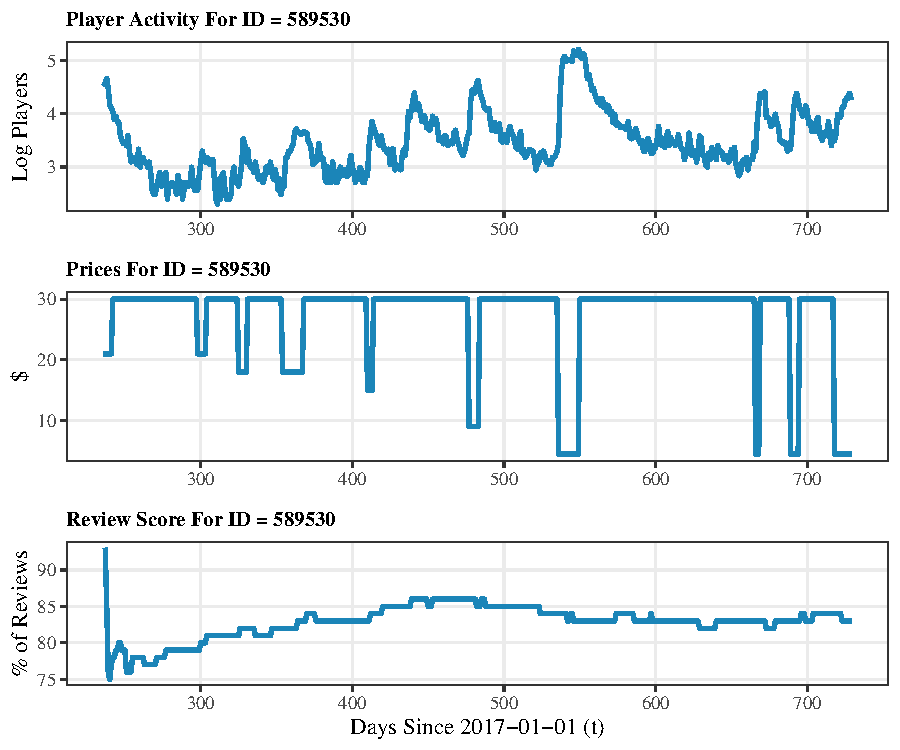
\includegraphics{/Users/dmitry/Steam_Discounting/Analysis/Output/Paper_files/figure-latex/example-game-1} 

}

\caption{\label{exampleGame} An Example Game in the Sample: Player Count, Price, and Review Score Histories.}\label{fig:example-game}
\end{figure}

Steam is home to more than 25,000 games that differ in their genres,
prices, sales, release dates, frequency of updates, and other
characteristics. Inevitably, an appropriate sample should be selected
for the analysis. \citet{SorokinStevens20} studies the causal effect of
reviews on sales on Steam, and I mirror closely the sample selection
procedure used in that paper. First, Steam has made some significant
changes to its review system in late 2016, and one of the effects was
the removal of the a big number of reviews from the review score
calculation. While it could be an intervention that is worthy of an
independent study, in practice combining the data from before and after
the intervention led to unsound results, so I focus on the two year
period from January 2017 to January 2019, keeping the review system as
stable as possible. In particular, only games that were released in this
time period make it to the sample.

Second, online multiplayer games and games that update frequently are
dropped from the sample, as these are products whose quality is changing
a lot over
time\footnote{Games on Steam have blogs that allow them to share news about updates with the audience. Publishing news about an update is voluntary, so it is possible that some games that continue to update after the release still made it to the sample.}.
Unobserved quality would present a big obstacle to the identification of
the effect of reviews on pricing decisions or sales, because, say, a
game that has just issued a major update might both upgrade to a better
review label (because of the positive reception of the new content) and
give a big discount to rekindle the interest of the players, but the
discounting decision would not be influenced by the review transition.
For the same reasons, I also drop free games and games that are released
in a beta-version (the so called ``Early Access'' program), as these
products are likely to be adding new content, and the update history is
not a perfect way to monitor the updating activity. Finally, I drop few
games with a player count of less than four on their median day, as
these games are simply very small, and the quality of their player count
data is questionable.

\hypertarget{sample-description}{%
\subsection{Sample Description}\label{sample-description}}

The final sample includes \texttt{r\ info{[},\ .N{]}} games which I
observe for
\texttt{r\ panel{[},\ max(age),\ by\ =\ ID{]}{[},\ round(mean(V1)){]}}
days each, on average. The main variables in the analysis are the
aforementioned dynamic variables: player count, price, and review score
history. An example observation from the sample is given in Figure
\ref{exampleGame}. For the majority of the games in the sample, the
player count is the highest around the release date, and then it quickly
fades away and oscillates around a smaller level. The player count also
jumps when a discount is given, reflecting the influx of new players.
Games differ a lot in their sizes, as is evident from Figure
\ref{sampleSizeHist}.

\begin{figure}[h]

{\centering 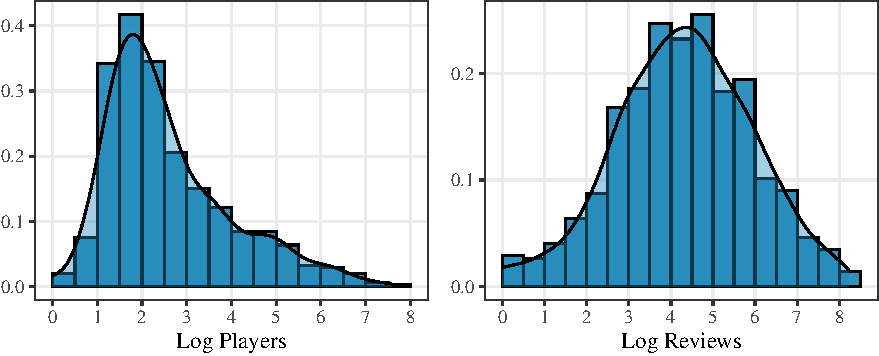
\includegraphics{/Users/dmitry/Steam_Discounting/Analysis/Output/Paper_files/figure-latex/sample-size-hist-1} 

}

\caption{\label{sampleSizeHist} Distributions of the Player Count on, and the Number of Reviews Accumulated by, the Age of 180 Days.}\label{fig:sample-size-hist}
\end{figure}

As the goal of the paper is to understand if firms use pricing tools in
order to improve their online reputation, a detailed overview of pricing
and review variables is important. A representative game in the sample
never changes its price, but instead occasionally goes on discounts,
slowly increasing their magnitude as the game ages. There are
\texttt{r\ panel{[}discount==F,\ diff(price),\ by\ =\ ID{]}{[}V1\textgreater{}0,\ .N{]}}
incidents of price change in the data, compared to
\texttt{r\ panel{[}discNew==T,\ .N{]}} discounts. Steam has a number of
rules that regulate price promotions on its platform. A game can have a
launch discount, but, otherwise, it has to wait for two months since the
release before changing its price or giving a discount. A game can not
go on discounts too frequently, and has to wait between four to six
weeks after a price promotion to be able to run a new one. The duration
of a custom discount is restricted to be at least one full day, and at
most two weeks. Besides these custom discounts, that are fully managed
by the firms, Steam has a series of curated discounts, when the platform
invites selected titles to go on a discount. As \citet{steamDiscounting}
explains it, ``while there aren't strict rules, as a base guideline we
tend to focus on the top 10-20\% selling games on Steam that are
positively reviewed and have otherwise proven to be successful''.
Curated promotions are featured prominently on Steam's main page, and,
arguably, lead to more visibility and sales for the participating titles
than custom discounts, which also contribute to visibility, but
typically do not get the front-page promotional slots. An important type
of curated discounts are the so-called ``Seasonal Sales''--big
platform-wide events that take place about four times a year around
major holidays. Figure \ref{seasonalSales} shows that the biggest sales
take place in Winter (Christmas and New Year) and Summer (July 4), but
there are also significant discounts in the Fall (Halloween and
Thanksgiving). Around
\texttt{r\ \ round(panel{[}discSeason==T\ \&\ discNew\ ==\ T,\ .N{]}/panel{[}discNew==T,\ .N{]}*100)}\%
of discounts in the sample go live during a Seasonal Sale. Thus, firms
have significant agency when it comes to running price promotions, but
platform regulations and platform-wide discounts are important
determinants of firms' decision to discount.

\begin{figure}[h]

{\centering 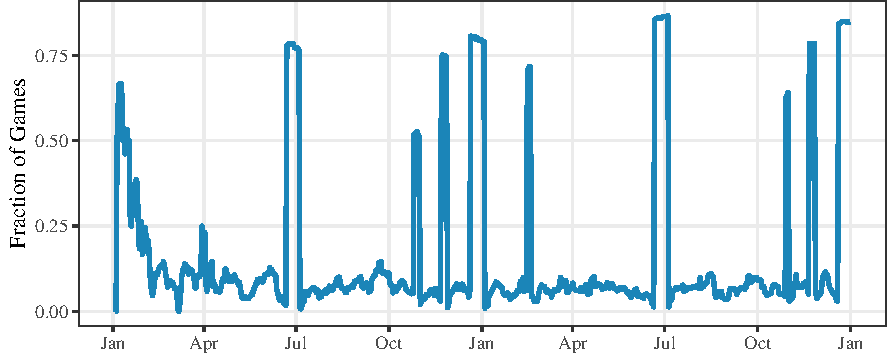
\includegraphics{/Users/dmitry/Steam_Discounting/Analysis/Output/Paper_files/figure-latex/seasonal-sales-1} 

}

\caption{\label{seasonalSales} Fraction of Games in the Sample Running a Promotion.}\label{fig:seasonal-sales}
\end{figure}

The path of the review score of a typical game is quite different from
its price history, in that the review score tends to settle quickly.
Recall that the review score is just the fraction of the positive
reviews among all reviews, so the law of large number implies that this
ratio crystallizes as more reviews flow in. Second plot in Figure
\ref{reviewDescriptivePlots} shows that games tend to receive half of
the reviews they have at the age of 180 days in their first month after
the release. On average across games, the standard deviation of the
review score (out of one hundred) is just
\texttt{r\ round(panel{[},\ sd(score,\ na.rm=T),\ by\ =\ ID{]}{[},\ mean(V1,\ na.rm\ =\ T){]},\ 2)},
with a split of
\texttt{r\ round(panel{[}age\ \textless{}=\ 30,\ sd(score,\ na.rm=T),\ by\ =\ ID{]}{[},\ mean(V1,\ na.rm\ =\ T){]},\ 2)}
in the first thirty days and
\texttt{r\ round(panel{[}age\ \textgreater{}\ 30,\ sd(score,\ na.rm=T),\ by\ =\ ID{]}{[},\ mean(V1,\ na.rm\ =\ T){]},\ 2)}
after that. The score is only assigned once the game reaches 10 reviews,
and once can see that 10 reviews is enough on average keep the score
stable. The distribution of games by bins at the age of 180 days,
depicted in Figure \ref{reviewDescriptivePlots}, is, then,
representative of the situation at other ages.

\begin{figure}[h]

{\centering 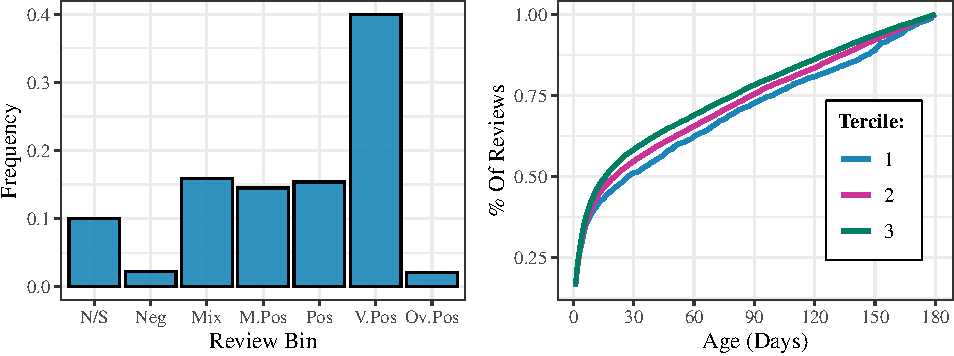
\includegraphics{/Users/dmitry/Steam_Discounting/Analysis/Output/Paper_files/figure-latex/review-descriptive-plots-1} 

}

\caption{\label{reviewDescriptivePlots} Distribution of Games by Review Bins and the CDF's of Review Arrival Times by Quintiles at 180 Days.}\label{fig:review-descriptive-plots}
\end{figure}

Despite the relative rigidity of the review score, there is enough
transitions between the review bins to make the analysis of pricing
decisions by firms around such transitions possible. Table
\ref{tab:transitionMatrix} describes the transitions between review bins
in the sample. The number of unique games that have changed review
labels in the data is
\texttt{r\ transitions{[},\ unique(ID){]}\ \%\textgreater{}\%\ length},
and the number of transitions is \texttt{r\ transitions{[},\ .N{]}}.
Sometimes games switch their bins briefly, and go back soon after. The
number of transitions that led to the game spending at least 7 days in
the new bin is
\texttt{r\ transitions{[}(is.na(dur)\ \textbar{}\ dur\ \textgreater{}=\ 7),\ .N{]}}.
Table \ref{mDiscountTable} describes the state of the games in the two
weeks before their transitions. Discounting does take place before the
transitions, games transition at very different ages, but tend to have
only a limited number of reviews by the time their review bin changes.

\begin{table}

\caption{\label{tab:transitionMatrix}Transition Probability And Count Matrices}
\centering
\resizebox{\linewidth}{!}{
\begin{tabular}[t]{ccccccccccccc}
\toprule
\multicolumn{6}{c}{Probabilities} & \multicolumn{1}{c}{ } & \multicolumn{6}{c}{Counts} \\
\cmidrule(l{3pt}r{3pt}){1-6} \cmidrule(l{3pt}r{3pt}){8-13}
Neg & Mix & M. Pos & Pos & V. Pos & Ov. Pos &   & Neg & Mix & M. Pos & Pos & V. Pos & Ov. Pos\\
\midrule
0 & 100 & 0 & 0 & 0 & 0 & Negative & 0 & 58 & 0 & 0 & 0 & 0\\
24 & 0 & 76 & 0 & 0 & 0 & Mixed & 60 & 0 & 189 & 0 & 0 & 0\\
0 & 43 & 0 & 25 & 33 & 0 & M. Positive & 0 & 245 & 0 & 141 & 188 & 0\\
0 & 0 & 40 & 0 & 60 & 0 & Positive & 0 & 2 & 207 & 0 & 310 & 0\\
0 & 0 & 84 & 0 & 0 & 16 & V. Positive & 0 & 0 & 220 & 0 & 0 & 43\\
0 & 0 & 0 & 0 & 100 & 0 & Ov. Positive & 0 & 0 & 0 & 0 & 25 & 0\\
\bottomrule
\end{tabular}}
\end{table}

\begin{table}[!htbp] \centering 
  \caption{Average Discount, Age, and Review Count Two Weeks Before A Transition} 
  \label{mDiscountTable} 
\begin{tabular}{@{\extracolsep{5pt}}lccccc} 
\\[-1.8ex]\hline 
\hline \\[-1.8ex] 
Statistic & \multicolumn{1}{c}{N} & \multicolumn{1}{c}{Mean} & \multicolumn{1}{c}{St. Dev.} & \multicolumn{1}{c}{Pctl(25)} & \multicolumn{1}{c}{Pctl(75)} \\ 
\hline \\[-1.8ex] 
Mean Discount (\%) & 1,225 & 10 & 14 & 0 & 15.9 \\ 
Age & 1,225 & 142 & 157 & 8 & 226 \\ 
Reviews & 1,225 & 130 & 343 & 26 & 81 \\ 
\hline \\[-1.8ex] 
\end{tabular} 
\end{table}

\begin{figure}[h]

{\centering 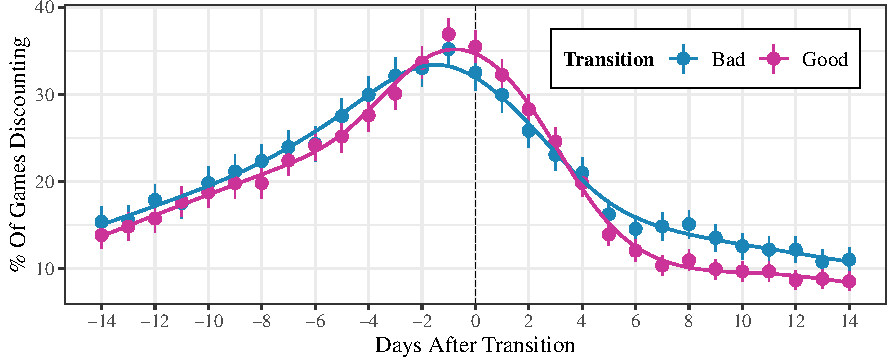
\includegraphics{/Users/dmitry/Steam_Discounting/Analysis/Output/Paper_files/figure-latex/transition-discount-plot-1} 

}

\caption{\label{discountsTransitions} Discounting By Games Around The Transition.}\label{fig:transition-discount-plot}
\end{figure}

\hypertarget{descriptive-evidence}{%
\section{Descriptive Evidence}\label{descriptive-evidence}}

In this section I present evidence that firms use discounting to manage
their online reputation, in particular, by running price promotions when
they are close to improving their review label. For now, let us resort
to a very simplistic story of why a firm would be interested in doing
that. Assume that discounts increase the inflow customers, and that more
customers means more reviews. Also, take for granted, for now, that
better review labels improve sales. Then, if a firm is one positive
review away from upgrading its review label, it might be tempted to
speed things up by giving a discount. Similarly, a product that is close
to sliding into a worse review bin, could be tempted to run a price
promotion, in order to avoid a slump in its reviews. I will address this
story in more detail in the discussion part of this section, but for now
I turn attention to simply establishing that this sort of behavior
indeed takes place in the sample.

The departing point of the analysis is Figure
\ref{discountsTransitions}, which shows that transitions between review
labels are very often preceded by discounts. The graph shows that two
weeks prior to a transition only 15\% of games were on a discount, a
number close to the sample average, but that this number more than
doubles to around 35\% one day before the label change. Regression
analysis controlling for review label, number of reviews, age, day of
the week and week time effects, as well as time since the previous
discount, confirms that the association depicted in Figure
\ref{discountsTransitions} is robust (see Table \ref{transitionReg} in
the Appendix). A game is approximately
\texttt{r\ round(reg1\$coefficients{[}2{]}*14*100)} pp more likely to be
on a discount on the day of the transition than it is two weeks prior to
it, and it is \texttt{r\ round(-reg1\$coefficients{[}3{]}*14*100)} pp
less likely to be on a discount two weeks following the transition.
Given that the probability for a game to be on a discount on a random
day is
\texttt{r\ round(panel{[},\ mean((discount\ \textgreater{}\ 0),\ na.rm=T){]}*100)}\%
in the sample, these effects amount to
\texttt{r\ round(100*(reg1\$coefficients{[}2{]}/panel{[},\ mean((discount\ \textgreater{}\ 0),\ na.rm=T){]}))}\%
and
\texttt{r\ round(100*(-reg1\$coefficients{[}3{]}/panel{[},\ mean((discount\ \textgreater{}\ 0),\ na.rm=T){]}))}\%
changes in the daily probability of a discount, which is quite sizable.

Of course, this finding simply shows a correlation between firms'
discounting behavior and review transitions. The same pattern could
emerge if the causality between the two variables is reversed, i.e.~the
discounts cause transitions, and not the other way around. Imagine a
hypothetical world in which games are only bought on discounts. In this
world any action in the data would be preceded (and, to some extent,
caused) by a discount. In other words, firms could be giving discounts
for reasons unrelated to reviews, but transitions sometimes would follow
as a result. As a matter of fact, suppose that the story I am after is
true, and that firms try to achieve transitions via price promotions. In
that case, discounts \emph{have} to be able to aid transitioning, making
the reverse causality inherent in this setting. The analysis behind
Figure \ref{discountsTransitions} remains imperfect for yet another
reason. A discount given when a firm is close to a positive transition
is not guaranteed to lead to a transition. Similarly, a firm trying to
avoid a negative transition by giving a discount might succeed. In both
cases, the behavior that we are interested in goes undetected if one
only studies transitions that took place in the data.

The solution to both problems that I suggest is to study
\emph{potential} transitional situations instead of the realized ones.
First, it solves the reverse causality problem. A discount given today
can cause a transition tomorrow, but a decision to give a discount can
not cause the proximity to a transition that chronologically precedes
it. Second, it clearly solves the selection issue explained above, when
the analysis considers solely the firms that transitioned.

With the focus now on potential transitions, the crucial question is how
to define proximity to a transition. One approach would be to use the
raw review count, and to say that a game is close to upgrading its
review label when it needs five (ten, twenty \ldots) more positive
reviews to transition. However, given the heterogeneity in the
popularity of different games (see Figure \ref{sampleSizeHist}), five
extra reviews could be nothing for a very popular game, and hard to
acquire for a small game. For this reason I use a different approach,
that measures proximity by the expected number of days that a game has
to wait to accumulate the reviews necessary for a transition. In
particular, for every game-date pair I first measure how many positive
reviews that game needs at the moment to upgrade its review bin, and how
many negative reviews that game needs to degrade its review bin. In the
next step, for each game I calculate the average speed of review
arrivals, by simply dividing the number of positive (negative) reviews
as of the last day in the sample by the age of the game on that day.
Knowing the speed of positive and negative review arrivals, and the
number of reviews necessary for a transition, I then define the
proximity to a positive (negative) transition to be the expected number
of days needed for the game to accumulate the necessary number of
positive (negative) reviews, assuming that it does not receive any
negative (positive) reviews during that time.

To illustrate this definition, consider an example game with 19 positive
reviews and 6 negative reviews at some moment in time. This game has a
review score of 76\%, and the ``Mostly Positive'' review label. It needs
5 additional positive reviews to secure a score of 80\%, the threshold
that would earn it the ``Positive'' label. Similarly, 3 new negative
reviews would be sufficient for the game to slide into the ``Mixed''
review category, as the score would become
\(19/(25 + 3) \times 100\%= 67\%\), which is less than the \(70\%\)
required for the ``Mostly Positive'' bin. If this game ends up having 80
positive and 20 negative reviews at the age of 200 days, its last day in
the sample, then, on average, it was receiving 0.4 positive and 0.1
negative reviews per day. Thus, for a positive transition it requires
\(5/0.4 = 12.5\) days of only good reviews arriving at this rate.
Similarly, for a negative transition it requires \(3 / 0.1 = 30\) days
of only bad reviews arriving at this rate. So, for this game I set its
proximity to a potential positive transition to be 12.5 days, and its
proximity to a potential negative transition to be 30 days.

As the example above shows, it is impossible to consider proximity to a
positive transition without taking into account the proximity to a
negative transition, at least for moderately sized games. If firms'
strategies for these types of transitions are different, then studying
such transitions separately could attenuate the effect of the proximity
to, say, a positive transition, on the discount probability: a firm that
is close to upgrading its review bin might not give a discount not
because it is a bad way to accomplish that transition, but because that
firm is at the same time close to downgrading its review bin, and might
prefer to exercise prudence. For this reason, I define two ``treatment''
variables of interest. Game \(i\) at date \(t\) is said to be close to a
positive transition, \(T_{it}^+ = 1\), if its proximity to a positive
transition is less than or equal to \texttt{r\ 2*band} days. Similarly,
game \(i\) at date \(t\) is said to be close to a negative transition,
\(T_{it}^- = 1\), if its proximity to a positive transition is less than
or equal to \texttt{r\ 2*band} days. The \texttt{r\ 2*band} cutoff is
inspired by the maximum duration of custom discounts on Steam, and the
patterns of discounting around successful transitions, depicted in
Figure \ref{discountsTransitions}. To estimate the effect of being close
to a review transition on the discounting behavior, I then estimate the
following model: \begin{equation}\label{potTransitionsReg}
disc_{it} = \beta^+ T_{it}^+ + \beta^- T_{it}^- + X_{it}\beta + f_i + \tau_t + \varepsilon_{it},
\end{equation}

\noindent \(disc_{it} = \mathds{1}\{Discount_{it} > 0\}\) is a dummy
measuring if the game is on a discount or not, \(X_{it}\) is a set of
control variables that includes log proximities to positive and negative
transitions, log review count, review bin dummies, and age; \(f_i\) is a
set of game-level fixed effects, and \(\tau_t\) is a set of day of the
week effects and sample week time effects. These time effects are
especially important to include in the regressions with discounting
variables on the left hand side, because Steam's curated discounts all
start on predetermined days of the week, and seasonal sales affect a big
number of games at the same time, as depicted in Figure
\ref{seasonalSales}. We expect \(\beta^+\) to be positive, but, when it
comes to \(\beta^-\), any sign could be rationalized. A positive sign on
\(\beta^-\) would serve as evidence that firms use discounting in order
to escape from slumps in their reviews bins, while a negative sign would
indicate that, on the contrary, firms on the verge of a bad transition
become more prudent with their discounts, trying to not instigate extra
purchasing/reviewing activity.

\begin{table}[hp] \centering    \caption{Discounts Close to Potential Transitions}    \label{potentialTransitionsResults}  \begin{tabular}{@{\extracolsep{5pt}}lccc}  \\[-1.8ex]\hline  \hline \\[-1.8ex]   & \multicolumn{3}{c}{\textit{Dependent variable:}} \\  \cline{2-4}  \\[-1.8ex] & \multicolumn{3}{c}{Discount Probability} \\   & Full & 1 W. to Tr. & Simple Tr. \\  \hline \\[-1.8ex]   Close to Pos. Transition & 0.010$^{***}$ & 0.009$^{***}$ & 0.007$^{***}$ \\    & (0.002) & (0.002) & (0.003) \\    Close to Neg. Transition & $-$0.008$^{***}$ & $-$0.002 & $-$0.007$^{***}$ \\    & (0.002) & (0.002) & (0.003) \\    Log Days to Pos. Tr. & 0.005$^{***}$ & 0.004$^{***}$ & 0.007$^{***}$ \\    & (0.001) & (0.001) & (0.001) \\    Log Days to Neg Tr. & $-$0.003$^{***}$ & $-$0.002$^{***}$ & $-$0.001 \\    & (0.001) & (0.001) & (0.001) \\    Log Reviews & $-$0.003$^{***}$ & $-$0.002$^{***}$ & $-$0.003$^{***}$ \\    & (0.001) & (0.001) & (0.001) \\    Mostly Positive & $-$0.008$^{***}$ & $-$0.009$^{***}$ & $-$0.007$^{***}$ \\    & (0.002) & (0.002) & (0.002) \\    Positive & $-$0.012$^{***}$ & $-$0.013$^{***}$ &  \\    & (0.002) & (0.002) &  \\    Very Positive & $-$0.008$^{***}$ & $-$0.007$^{***}$ &  \\    & (0.002) & (0.002) &  \\    Age & 0.0001$^{***}$ & 0.0001$^{***}$ & 0.0001$^{***}$ \\    & (0.00000) & (0.00000) & (0.00001) \\    Age $\le 14$ & 0.050$^{***}$ & 0.049$^{***}$ & 0.018$^{*}$ \\    & (0.005) & (0.005) & (0.009) \\   \hline \\[-1.8ex]  Time Effects: Weekdays, Week &  $\checkmark$ &  $\checkmark$ & $\checkmark$ \\ Game Effects & $\checkmark$ & $\checkmark$ & $\checkmark$ \\ Poly($t$ W/O Discount, $d=2$) & $\checkmark$ & $\checkmark$ & $\checkmark$ \\ Observations & 295,228 & 295,228 & 113,901 \\  R$^{2}$ & 0.172 & 0.172 & 0.173 \\  \hline  \hline \\[-1.8ex]  \textit{Note:}  & \multicolumn{3}{r}{$^{*}$p$<$0.1; $^{**}$p$<$0.05; $^{***}$p$<$0.01} \\  \end{tabular}  \end{table}

Notice that the inclusion of both the distance to a potential positive,
and a potential negative, transition in the regression drops all
observations from the lowest (``Negative'') and the highest
(``Overwhelmingly Positive'') review bins, as for games in those bins
only one way of review transition is possible. However, given that the
proportion of such observations in the sample is quite small, this is
not a big concern. The analysis also excludes the observations with a
``No Review Score'' label, as I do not want to take a stance on what
constitutes an improvement or a deterioration of the review score for
such games. The results of estimating Equation \ref{potTransitionsReg}
are presented in Table \ref{potentialTransitionsResults}. The first
column is the full specification that uses all observations in the
sample (except the omissions just mentioned). The second column uses a
more stringent definition of proximity to a transition, requiring a game
to be \texttt{r\ band}, rather than \texttt{r\ 2*band}, days away from a
potential transition to be counted as being ``close to a transition''.
The third column uses only transitions between ``Mixed'', ``Mostly
Positive'', and ``Positive'' labels, as these are the transitions that
rely on the review score only, while ``Very Positive'' and
``Overwhelmingly Positive'' require both a certain review score, and a
certain number of
reviews.\footnote{Technically, a game improving its review score from 79\% to 80\% can transition to both “Positive” and “Very Positive”, so the results in the third column bundle together these types of transitions.}.
\citet{SorokinStevens20} exclusively uses these simple review bins in
their regression discontinuity analysis, precisely in order to avoid the
complications that arise from double thresholds required for ``Very
Positive'' and ``Overwhelmingly Positive''.

The results in Table \ref{potentialTransitionsResults} unequivocally
support the hypothesis that proximity to a review bin upgrade increases
firms' willingness to run a price promotion. Measured against the
\texttt{r\ round(panel{[},\ mean((discount\ \textgreater{}\ 0),\ na.rm=T){]}*100)}\%
probability for a random game-day pair from the sample to have a
discount\textbackslash footnote\{The corresponding number for the games
in the treatment group is
\texttt{r\ round(100*panel{[}ID\ \%in\%\ panel{[}pos.treatment\ ==\ 1,\ unique(ID){]},\ mean((discount\ \textgreater{}\ 0),\ na.rm\ =\ T){]})}.\},
the effects constitute a
\texttt{r\ round(100*(reg3\$coefficients{[}1{]}/panel{[},\ mean((discount\ \textgreater{}\ 0),\ na.rm=T){]}))}-\texttt{r\ round(100*(reg1\$coefficients{[}1{]}/panel{[},\ mean((discount\ \textgreater{}\ 0),\ na.rm=T){]}))}\%
increase in the daily probability of a discount. The uncertainty about
the sign and the significance of the proximity to a potential negative
transition is resolved in favor of the prudent approach on the firms'
side: the results suggest that firms under a risk of deteriorating their
review label are
\texttt{r\ -round(100*(reg3\$coefficients{[}2{]}/panel{[},\ mean((discount\ \textgreater{}\ 0),\ na.rm=T){]}))}-\texttt{r\ -round(100*(reg1\$coefficients{[}2{]}/panel{[},\ mean((discount\ \textgreater{}\ 0),\ na.rm=T){]}))}\%
less likely to go on a discount, albeit the effect is only present in
two out of three specifications.

\hypertarget{discussion}{%
\subsection{Discussion}\label{discussion}}

It is not unreasonable to say that model \ref{potTransitionsReg} is able
to identify the causal effect of the proximity to a review transition on
discounting behavior. As the sample was selected to include only
products with the most stable quality and the lowest number of game
updates, the path of the review score is relatively exogenous for the
firms. Taking its current review score as given, a firm can decide
whether to run a price promotion or not, which makes the main
independent variables in my analysis exogenous. On top of that, model
\ref{potTransitionsReg} includes a rich set of controls and fixed
effects. Some threats to identification still remain, of course. One is
unobserved marketing interventions preceding discounts. If
advertisements improves the review score, then, by definition,
advertisement would be correlated with the treatment variable, moving
games a bit closer to transitions. If a discount then follows, as a part
of the general marketing plan, rather than to leverage the new proximity
to a transition, the positive association between discounting and
positive transitions would be spurious. Note, however, that it would be
more natural to expect firms to roll out all marketing interventions at
the same time (i.e., running a price promotion while the game is
advertised). In that case, the threat to identification vanishes.

I would now like to step back and look at the story behind the behavior
that I am documenting. Several gaps are not filled yet. First, I have
not presented evidence that discounting meaningfully increases sales and
leads to more reviews. Neither have I presented evidence that better
review bins increase sales. Perhaps, more importantly, I have not
discussed why firms should expect customers buying during a discount to
leave better reviews than customers paying the regular price. If there
is no difference between the two groups, then giving a discount when the
game is close to a transition is, at best, a gamble. In fact, there is
some empirical evidence that customers who choose to go to a restaurant
because of a promotion tend to leave worse reviews
\citep{ByersEtAl12, Li16}, even though the effect could be positive in
certain cases \citep{Li16, ZhuEtAl19}. Theoretically, this effect is
ambiguous. Consumers who buy when the price is low could be a worse
match for the product and, thus, leave worse reviews. At the same time,
such customers get a higher utility from paying less, which, together
with a desire to reciprocate, can lead them to leave better reviews.
See, for example, \citet{AcemogluEtAl19}.

The results I presented in this section, therefore, lead to the
following hypotheses. I show that firms give discounts to avoid bad
transitions and to facilitate the good ones; thus, it has to be the case
that the reviews left on a discount tend to be more positive than the
ones left off a discount. Second, if that is indeed the case, then the
firms that get especially positive reviews during price promotions
should be more likely to try to use discounting to manipulate their
reviews. Heterogeneity between the firms is crucial for the second
hypothesis. In order to test these hypotheses, and to provide evidence
on the effect of discounting on sales and reviewing activity, as well as
the effect of reviews on sales, I now turn to formulation and estimation
of a structural model demand, reviewing and gaming activity on Steam.

\hypertarget{empirical-model}{%
\section{Empirical Model}\label{empirical-model}}

\hypertarget{setup}{%
\subsection{Setup}\label{setup}}

Consider game \(i\) that is observed on a daily basis. On day \(t\) the
game sells one copy to each of the \(B_{it}\) short-lived buyers that
arrive on that day, a number that is unobserved by the econometrician.
Define \emph{active players} of this game, \(A_{it}\), to be the
customers who have already purchased the game and are still playing it,
either because they have not yet completed it or are not bored with it
yet. This number has an empirical counterpart in the face of the player
count variable, observable to the econometrician. The game loses
\(E_{it}\) players on day \(t\), which is also not observed. I assume
that, once a player stops playing the game, she never returns to it
again. It is easy to see then that \(A_{it}\) follows the following
process: \begin{equation}\label{activeProccess}
  A_{it} = A_{it-1} + B_{it} - E_{it}
\end{equation}

Both the arrival of buyers and the exit of players are not observed, so
some assumptions need to be made about them in order to make progress.

\begin{assumption}\label{arrivalAssumptions}
$B_{it}$ is Poisson with arrival rate $\lambda_{it} = \lambda_i(1+x'_{it}\beta)$, where $x_{it}$ is a vector of observable characteristics of the game, and $\lambda_i$ and $\beta$ are parameters. $E_{it}$ follows a binomial distribution $B(A_{it-1}, 1-\psi_i)$, where $\psi_i$ is a parameter.
\end{assumption}

The rationale behind assumption (\ref{arrivalAssumptions}) is simple.
Consumers arrive every day according to the game specific arrival rate
\(\lambda_i\), but that rate can go up or down depending on the values
of observable characteristics \(x_{it}\) of the game that affect demand:
price, reviews, age of the game, or seasonal factors. The mapping
between these variables and the number of copies sold is, of course,
nothing else but the demand curve for game \(i\). A change of \(0.01\)
in the index \(x_{it}'\beta\) means that quantity demanded of game \(i\)
goes up by one percent. This multiplicative structure is necessary,
because it will allow me to estimate the price sensitivity and the
effect of reviews on sales in relative
terms\footnote{See the Identification section for more details}. Buyers
of the game become active players, and are subject to a fixed daily risk
of \(1-\psi_i\) of abandoning the game. Given that the number of active
players ``flipping'' this coin at the end of day \(t-1\) is
\(A_{it-1}\), this process gives rise to the binomial distribution for
the number of exiters.

Every buyer of game \(i\) is a potential reviewer. I assume that a buyer
who buys the game at \(t-k\) leaves a positive (negative) review for the
game on day \(t\) with probability \(r_{it}^+\) (\(r_{it}^-\)), and no
review otherwise. For the reasons I will explain later, I will refer to
\(r_{it}^+\) as the \emph{like rate}, and to \(r_{it}^-\) as the
\emph{dislike rate}. The focus of the analysis is on the difference
between the reviews left on and off a discount. To that end, I
parametrize the like and dislike rates to depend on the discounting
behavior of the firm as follows.

\begin{assumption}\label{likeDiscountAss}
The like rate is a linear function of discounts:
$r_{it}^+ = \rho_{0i}^+ + \rho_{1i}^+ disc_{it-k}$.  The dislike rate is a linear function of discounts: $r_{it}^- = \rho_{0i}^- + \rho_{1i}^- disc_{it-k}$.
\end{assumption}

\noindent Notice, that a price change affects the reviewing behavior in
two ways. First, a lower prices increases the inflow of buyers through a
higher \(\lambda_{it}\). This leads to more reviews being left. My
parametrization allows to further study if the reviewers who bought the
game on a discount are more or less likely to leave positive and
negative reviews. I use a dummy variable \(disc_{it-k}\) to measure
discounting because this will allow me to derive a closed-form estimator
for the parameters of interest.

\hypertarget{identification}{%
\subsection{Identification}\label{identification}}

\hypertarget{demand-parameters}{%
\subsubsection{Demand Parameters}\label{demand-parameters}}

The prediction of \(A_{it}\) that follows from (\ref{activeProccess})
takes the form of \begin{equation}
\mathbb{E}\left[A_{it}\,|\,A_{it-1}, x_{it} \right] = A_{it-1} + \lambda_i(1+x'_{it}\beta) - (1-\psi_i)A_{it-1} = \psi_i A_{it-1} + \lambda_i(1+x'_{it}\beta),
\end{equation} so the model implies the following regression equation
\begin{equation}\label{arrivalReg}
 A_{it} = \psi_i A_{it-1} + \lambda_i(1+x'_{it}\beta) + u_{it},
\end{equation} with
\(\mathbb{E}\left[u_i\,|\,A_{it-1}, x_{it} \right] = 0\). This model is
non-linear in parameters, because \(\lambda_i\) is not known and enters
the model multiplying \(\beta\), the parameters common to all games. If
not for this commonality in \(\beta\), estimation of (\ref{arrivalReg})
would be straightforwardly achieved by opening the parentheses and
estimating \begin{equation}\label{arrivalRegInd}
A_{it} = \lambda_i + \psi_i A_{it-1} + x'_{it}\beta_i + u_{it}
\end{equation} using OLS on a game-by-game basis. This commonality is
essential, however, because one game in the sample typically does not
exhibit enough variation in review labels to be able to identify the
effect of upgrading the review tier on sales.

The fact that \(x'_{it}\beta\) multiplies the game fixed effect
\(\lambda_i\) allows me to estimate the dependence of quantity sold on
price and reviews in relative terms, i.e., to obtain the elasticities.
Normally, a log transformation is used to achieve that. Indeed,
\citet{SorokinStevens20} is able to estimate these elasticities with a
within-estimator, using the following model
\begin{equation}\label{logReg}
\log A_{it} = \tilde\lambda_i + \tilde\psi_i \log A_{it-1} + x'_{it}\tilde \beta + u_{it}.
\end{equation} This specification ``controls'' for the (log) number of
continuing players in order to overcome the non-availability of direct
sales data; however, it is the numbers of active players and buyers that
are additive, not their logs. Thus, the structural model I formulate
confronts the estimation problem in a more ``heads-up'' way, and in that
regard offers an improvement over \citet{SorokinStevens20}. I will
contrast the results obtained by the two approaches in the results
section, comparing a more detailed structural approach with a less
precise, but a more easily implementable, log regression approach.

Another important reason for insisting on estimating the relative
effects stems from the limitations of my data. Recall that the player
count variable measures only the \emph{maximum concurrent} number of
active players every day. This implies that the estimated values of
\(\lambda_{it}\) would take into account only those new buyers who
contribute to gaming activity during the ``rush hour''. An implicit
assumption in my analysis is that new buyers of the game all choose
their gaming time following the same game-specific distribution. I use
this assumption to say that, if the number of new active players during
rush hour goes up by 1\%, then sales go up by 1\% across all types of
players, not only among the ``rush hour ones''.

Assumption \(\mathbb{E}\left[u_i\,|\,A_{it-1}, x_{it} \right] = 0\)
holds by definition for Model \ref{arrivalReg}, and guarantees
identification of all parameters, as long as there is sufficient
variation in the data. Of course, this is only true as long as equation
\ref{arrivalReg} is the right model of the data generating process. A
threat to identification would come from unobserved demand shifters
\(\tilde x_{it}\) that are correlated with the observed factors
\(x_{it}\) (omitted variable bias). For instance, an advertising
intervention that is coupled with a price promotion would increase
demand, but the entire effect would be attributed to the observed change
in price. My approach is vulnerable to such events, as long as one is
interested in getting the causal estimate of the discount elasticity of
demand.

However, I argue that (\ref{arrivalReg}) is an adequate specification,
if the goal is to estimate the causal effect of reviews on sales, or to
get a predictive model of demand. First and foremost, the reviews are
not a choice variable of a firm, and rather serve as a state variable
that a firm takes as given every day. Of course, there are various
things that a firm can do, that can, in a non-guaranteed fashion, affect
this variable. But, as long as the major tools that a firm has access to
are controlled for in the regression, the exogenous variation in the
review variables is sufficient to identify the causal effect of reviews
on sales.

One important way in which I control for various tools that firms have
at their disposal is through sample selection. Sample selection rules
out the possibility of an omitted variable bias stemming from a number
of variables that could collectively be referred to as ``changing
quality''. The games in the sample are single player games, and thus are
not subject to time-varying network externalities or frequent quality
updates, that could be correlated with reviews, depths of discounts, and
the player count. Second, game specific effect \(\lambda_i\) controls
for all time-invariant characteristics of game \(i\) that determine
average sales: initial marketing budget, extraneous popularity of the
game's plot or setting, etc. Similarly, time effects control for
important within-week seasonality in gaming patterns and for the
extensive platform-wide sales. Third, note that Equation
(\ref{arrivalReg}) allows each game to have its own continuation
probability \(\psi_i\), which could prove crucial in eliciting sales
from the player count data. Two games could have the same observed
median daily player count---say, ten people---but very different sales
levels, if game one offers a lot of replayability and is played by the
same ten people over and over again, and game two is played by new ten
people every day. Intuitively, \(\psi_i\) is identified by the rate of
decay of the player count when it is far from its (slowly-changing)
trend or average. Game release and discounts offer such events, when the
player count spikes briefly due to all the new players who just bought
the game; see example game in Figure \ref{exampleGame}.

\hypertarget{price-elasticity-of-demand}{%
\subsubsection{Price Elasticity of
Demand}\label{price-elasticity-of-demand}}

To close off the discussion of identification of the demand parameters
in Equation (\ref{arrivalReg}), I would like to elaborate on the
identification of the price elasticity parameter. As I mentioned before,
at the very least, including the price in the regression controls for
unobserved marketing interventions that are coupled with discounts.
Estimating the true price elasticity of demand is not important for the
questions addressed in this paper, as I am not trying to prescribe the
sizes of the discounts that firms should be giving to have a meaningful
chance of affecting their review labels when they are close to a review
transition. Arguably, a 100\% discount is a powerful enough option to
make this strategy viable, at least in principle. However, should the
price coefficient be of primary interest, I would like to list some
further factors that have an impact on the identification of thereof.

First, I believe that standard concerns about the endogeneity of prices
are not directly applicable in my context. The reason is the high
frequency nature of the data and the stickiness of posted prices. Using
the classic notation, imagine that a discount is given on date \(t\),
and we observe a quantity-price pair \((Q_t, P_t)\), both of which are
different from their yesterday's counterparts \((Q_{t-1}, P_{t-1})\).
The standard endogeneity concern is that firm's demand is subject to
shocks, and that the firm would change its price precisely when those
shocks occur. The two points then, roughly speaking, would belong to
different demand curves, and one can not identify the slope of the
demand
curve\footnote{Assuming, as is usually done, that demand shifters lead to parallel shifts in demand}.
In my setting, however, this would require the firms to systematically
give discounts \emph{exactly on the days} of the demand shocks, which
requires possessing a level of insight into one's demand condition that
is unrealistic, especially for small independent studios. While a
discount for a racing game on the day of a major F-1 race is not
implausible, should the demand for the game go up with a lag of as
little as one day, then both \((Q_t, P_t)\) and \((Q_{t-1}, P_{t-1})\)
would belong to the same demand curve, and, therefore, identification
would not be threatened.

My second point is that, even though unobserved marketing interventions
that are coupled with price promotions, would, undoubtedly, be an issue,
this problem could be addressed with some extra data collection. One way
to proceed would be to study if such coupled promotions in fact do take
place. In particular, one could collect data on YouTube queries
mentioning the games in the sample, and use spikes in such queries as a
proxy for unobserved marketing campaigns.

A deeper problem for identifying the price elasticity of demand lies in
defining precisely the elasticity of interest. A video game is a durable
good, and some consumers could be purchasing it strategically, thinking
about the probability and depth of discounts that they could get in the
near future. A discount that is announced a week in advance will appear
to have a strong effect on sales, but only because consumers would
abstain from purchasing the game throughout that week. For studying
counterfactual price policies one would need to specify a more
complicated model of forward-looking consumers, and estimate the
fundamentals of their behavior. A related problem is the importance of
salience in a marketplace that has many thousands of products. Any price
elasticity estimated relies on Steam keeping its algorithms unchanged. A
game can give a 99\% discount, but the quantity demanded will not change
much if that promotion happens to not be reflected in Steam's system.
This has implications, for instance, for picking good instruments for
prices. Curated discounts created and managed by Steam are suggested to
firms, and not chosen by them. In principle, such price changes could be
exogenous to daily demand conditions. However, they could hardly be used
as instruments for the price, because they also bring an immense boost
in visibility, by the virtue of occupying the prime store main page
space.

\hypertarget{review-parameters}{%
\subsubsection{Review Parameters}\label{review-parameters}}

The part of the model describing the reviewing behavior of the buyers is
more starightforward. Intuitively, the propensity to leave a review on
and off a discount (the like and dislike rates \(r_{it}^+\),
\(r_{it}^-\)) are identified by the differences in reviews left on and
off a discount. In fact, this intuition becomes a rigorous proof, as wil
be shown shortly.

Following assumption \ref{arrivalAssumptions}, the arrival of buyers for
game \(i\) on day \(t\) follows a Poisson distribution with arrival rate
\(\lambda_{it} = \lambda_i (1 + x_{it}'\beta)\). I also assumed that,
\(k\) days later, each consumer leaves a positive review with
probability \(r_{it}^+\), a negative review with probability
\(r_{it}^-\), and no review otherwise. Then, the following proposition
is true:

\begin{proposition}\label{poissonReviews}
The number of good reviews $G_{it}$ for game $i$ on day $t$ is distributed Poisson with rate $r_{it}^+\lambda_{it-k}$. The number of bad reviews $B_{it}$ for game $i$ on day $t$ is distributed Poisson with rate $r_{it}^-\lambda_{it-k}$. Moreover, $G_{it}$ and $B_{it}$ are independent.
\end{proposition}

Proposition \ref{poissonReviews} allows one to easily write down the
likelihood for positive and negative reviews separately. I will use the
positive reviews as the leading example here, but all the findings
automatically translate to the negative reviews case as well. For every
game I observe the history of the review arrivals
\(\{(g_{it}, b_{it})\}_{t=1}^{T_i}\). Since
\(\PP{G_{it} = g_{it}} = \frac{ (r_{it}^+\lambda_{it-k} )^{g_{it}} }{g_{it}!} e^{ -r_{it-k}^+\lambda_{it-k} }\),
the log-likelihood of the history of likes is given by
\begin{equation}\label{reviewsLikelihood}
\ell(g_i; r_{it}^+, \lambda_{it-k}) = \sum_{t\ge k} g_{it} \log r_{it}^+\lambda_{it-k} - r_{it}^+\lambda_{it-k} - \log g_{it}!
\end{equation}

I treat \(\lambda_{it}\) as known, because parameters \(\lambda_{i}\)
and \(\beta\) that determine it can be estimated consistently for the
majority of games in the sample, given the long time dimension of the
panel. For now I also take the lag \(k\) between the time when the user
buys the game and leaves a review for the game to be known. The
parameters of interest are \((\rho_{0i}^+, \rho_{1i}^+)\), which
parametrize the like rate as
\(r_{it}^+ = \rho_{0i}^+ + \rho_{1i}^+ disc_{it-k}\). The likelihood is
concave in the parameters, so the parameters are identified as the
maximizer of the likelihood. Restricting attention to a binary discount
variable \(disc_{it}\) allows me to derive a closed-form estimator for
\((\rho_{0i}^+, \rho_{1i}^+)\). During a discount the like rate of game
\(i\) is \(\rho_{0i}^+ + \rho_{1i}^+\), which is consistently estimated
as \begin{equation}\label{rhohat1}
\hat \rho_{0i}^+ + \hat\rho_{1i}^+ = \frac{\sum_{t \ge k} disc_{it-k}g_{it}}{\sum_{t\ge k} disc_{it-k}\lambda_{it-k}},
\end{equation} As we can see, the ML-estimator of the like rate during a
price promotion is just the ratio of the number of good reviews left on
a discount over the expected arrival on that day. Similarly, the like
rate off a discount can be estimated by \begin{equation}\label{rhohat2}
\hat \rho_{0i}^+ = \frac{\sum_{t\ge k} (1-disc_{it-k})g_{it}}{\sum_{t\ge k} (1-disc_{it-k})\lambda_{it-k}},
\end{equation} with the interpretation that the like rate in the absence
of a discount is just a ratio of the reviews left outside of a discount
and the expected number of customers outside a discount.

Note that one can use these estimators to estimate the \emph{average
review score} on and off a discount, i.e., whether users are relatively
more or less likely to leave a good review during a discount. For
example, without a price promotion, one obtains
\begin{equation}\label{avReviewScore}
\frac{\sum_{t\ge k} (1-disc_{it-k})g_{it}}{\sum_{t\ge k} (1-disc_{it-k})g_{it} + \sum_{t\ge k} (1-disc_{it-k})b_{it}}
=
\frac{\hat \rho_{0i}^+}{\hat \rho_{0i}^+  + \hat \rho_{0i}^- }
\end{equation} It is intuitively clear that the relative propensity to
leave a good, rather than a bad, review should be easily estimable by
comparing the ratios of good to bad reviews, without any knowledge of
the quantity of games sold. This intuition is fully reflected in
Equation (\ref{avReviewScore}), where the arrival rates
\(\lambda_{it-k}\) have disappeared entirely.

The analysis above is complicated by two facts. First, for each game I
observe the exact review count, but my demand estimates only apply to
rush hours. If, say, every player leaves a review, and every day there
are two new players who play in the morning, and three new players who
play in the evening, my data would register 3 players leaving 5 reviews
on a daily basis. This is the reason why I refer to the values of
\((r_{it}^+, r_{it}^-)\) as rates, rather than probabilities (which they
are in the model). Propositon \ref{poissonReviews}, stating that the
number of good reviews on day \(t\) for game \(i\) is a Poisson random
variable with rate \(r_{it}^+\lambda_{it-k}\), could be treated as an
assumption, rather than a result. In that case, nothing constrains the
\(r_{it}^+\) parameter to be less than 1, and the identification
argument goes through in the exactly the same way.

Another problem stems from the fact that the purchase date behind a
review is not available to the researcher. For that reason, the model
features an additional parameter \(k\), the lag between purchasing the
game and leaving a review, that I assumed to be known. To estimate that
parameter I leverage the fact that spikes in player activity on the
first day of a sale represent new users, and study the review response
during the following week in order to uncover the modal lag for leaving
a review (see Table \ref{reviewLag} in the Appendix). This number turns
out to be one day. Even though time to posting a review has a
non-degenerate distribution, modelling it in a more nuanced way would
significantly contribute to complexity: the likelihood of receiving a
poisitive review on day 100 would depend on the entire history of buyer
arrivals prior to that date. Therefore, I proceed using \(\hat k = 1\).

\hypertarget{estimation-and-results}{%
\subsection{Estimation and Results}\label{estimation-and-results}}

\hypertarget{demand-parameters-1}{%
\subsubsection{Demand Parameters}\label{demand-parameters-1}}

\hypertarget{review-parameters-1}{%
\subsubsection{Review Parameters}\label{review-parameters-1}}

\newpage
\appendix

\hypertarget{additional-tables-and-figures}{%
\section{Additional Tables and
Figures}\label{additional-tables-and-figures}}

\hypertarget{discounts-around-transitions}{%
\subsection{Discounts Around
Transitions}\label{discounts-around-transitions}}

\begin{table}[hp] \centering    \caption{Discounts In The Days Around Transition}    \label{transitionReg}  \begin{tabular}{@{\extracolsep{5pt}}lc}  \\[-1.8ex]\hline  \hline \\[-1.8ex]   & \multicolumn{1}{c}{\textit{Dependent variable:}} \\  \cline{2-2}  \\[-1.8ex] & Discount Probability \\  \hline \\[-1.8ex]   Days to Transition & 0.006$^{***}$ \\    & (0.0005) \\    Days After Transition & $-$0.011$^{***}$ \\    & (0.0005) \\    No Score & 0.181$^{***}$ \\    & (0.026) \\    Negative & 0.004 \\    & (0.010) \\    Mostly Positive & $-$0.001 \\    & (0.005) \\    Positive & 0.032$^{***}$ \\    & (0.007) \\    Very Positive & 0.001 \\    & (0.006) \\    Ov. Positive & 0.004 \\    & (0.013) \\    Log Reviews & $-$0.011$^{***}$ \\    & (0.002) \\    Age & 0.0003$^{***}$ \\    & (0.00001) \\    Const & 0.872$^{***}$ \\    & (0.014) \\   \hline \\[-1.8ex]  Time Effects & Weekdays, Week \\ Game Effects & $\times$ \\ Polynomial($t$ W/O Discount) & $d = 2$ \\ Observations & 32,412 \\  R$^{2}$ & 0.397 \\  \hline  \hline \\[-1.8ex]  \textit{Note:}  & \multicolumn{1}{r}{$^{*}$p$<$0.1; $^{**}$p$<$0.05; $^{***}$p$<$0.01} \\  \end{tabular}  \end{table} 
\newpage

\hypertarget{review-lag}{%
\subsection{Review Lag}\label{review-lag}}

Table \ref{reviewLag} presents the results of estimating
\[NewReviews_{it} =\sum_{l = 0}^{7} \mathds{1}(\text{Disc. } l \text{ days ago})
+ reviewBin_{it} + age_{it} + young_{it} +  f_i + \tau_t + u_{it}\]

\begin{table}[hp] \centering    \caption{Spikes in Reviews After a Discount}    \label{reviewLag}  \begin{tabular}{@{\extracolsep{5pt}}lc}  \\[-1.8ex]\hline  \hline \\[-1.8ex]   & \multicolumn{1}{c}{\textit{Dependent variable:}} \\  \cline{2-2}  \\[-1.8ex] & New Reviews \\  \hline \\[-1.8ex]   Discount 0 Days Ago & 1.107$^{***}$ \\    & (0.123) \\    Discount 1 Day Ago & 3.308$^{***}$ \\    & (0.277) \\    Discount 2 Days Ago & 1.397$^{***}$ \\    & (0.139) \\    Discount 3 Days Ago & 0.748$^{***}$ \\    & (0.110) \\    Discount 4 Days Ago & 0.612$^{***}$ \\    & (0.096) \\    Discount 5 Days Ago & 0.397$^{***}$ \\    & (0.104) \\    Discount 6 Days Ago & 0.036 \\    & (0.086) \\    Discount 7 Days Ago & $-$0.160$^{**}$ \\    & (0.073) \\   \hline \\[-1.8ex]  Time Effects & Weekdays, Week \\ Game Effects & $\checkmark$ \\ Observations & 355,983 \\  R$^{2}$ & 0.054 \\  \hline  \hline \\[-1.8ex]  \textit{Note:}  & \multicolumn{1}{r}{$^{*}$p$<$0.1; $^{**}$p$<$0.05; $^{***}$p$<$0.01} \\  \end{tabular}  \end{table}

\newpage

\hypertarget{mathematical-appendix}{%
\section{Mathematical Appendix}\label{mathematical-appendix}}

\hypertarget{proofs}{%
\subsection{Proofs}\label{proofs}}

\textbf{Proposition} \ref{poissonReviews}. Let the total number of
reviewers during a day, \(R\), be distributed Poisson with rate
\(\lambda\), \(R\sim P(\cdot; \lambda)\). A reviewer leaves a good
review with probability \(\pi\), and a bad review with probability
\(1-\pi\). Then, the numbers of good and bad reviews, \(G\) and \(B\),
are independent Poisson random variables with rates \(\pi\lambda\) and
\((1-\pi)\lambda\).

In the main text I have a Poisson arrival of customers, and only a
fraction of them become reviewers, but the same proof goes through with
that modification as well. The independence between the numbers of good
and bad reviews is the surprising part of the proposition, and it is
better highlighted in the form presented here.

\vspace{1em}

\noindent *Proof*: We start by showing that \(G\) is Poisson. \[
\PP{G=g} = \sum_{n=g}^{\infty}\CP{G = g}{R=n}\PP{R = n} 
=
\sum_{n = g}^{\infty}
\frac{n!}{g!(n-g)!}
\pi^g (1-\pi)^{n-g}
\frac{\lambda^n}{n!} e^{-\lambda}
\]

\noindent We leave only the parts that depend on \(n\) within the sum:
\[
e^{-\lambda}\frac{\pi^g}{g!}\sum_{n = g}^{\infty}
\frac{(1-\pi)^{n-g} \lambda^n}{(n-g)!}
=
e^{-\lambda}\frac{\pi^g\lambda^g}{g!}\sum_{n = g}^{\infty}
\frac{(1-\pi)^{n-g} \lambda^{n-g} }{(n-g)!}
=
e^{-\pi\lambda}\frac{\pi^g\lambda^g}{g!}\sum_{k=0}^{\infty}
\frac{[(1-\pi)\lambda]^{k} }{k!}e^{-(1-\pi)\lambda}
\]

\noindent The sum we have is just
\(\sum_{k=0}^{\infty} P(k; \lambda) = 1\), so the answer is \[
\PP{G=g} = \frac{[\pi\lambda]^g}{g!}e^{-\pi\lambda} = P(g; \pi\lambda)
\]

Now the independence part. We are interested in \(\PP{G=g, B=b}\), which
could be written as \[\PP{G=g, B=b} = \CP{G=g, B=b}{R=g+b}\PP{R=g+b} = 
\frac{(g+b)!}{g!b!}
\pi^g (1-\pi)^b
\frac{\lambda^{g+b}}{(g+b)!} e^{-\lambda}
\] Simply write \(e^{-\lambda} = e^{-\pi\lambda}e^{-(1-\pi)\lambda}\),
and collect the terms with \(g\) and with \(b\) to get \[
\PP{G=g, B=b} = 
\frac{\pi^g \lambda^g}{g!}e^{-\pi\lambda}
\frac{(1-\pi)^b\lambda^b}{b!}e^{-(1-\pi)\lambda}
=
P(g; \pi \lambda) P(b; (1-\pi)\lambda)\]

\begin{flushright}
$\triangleleft$
\end{flushright}

\newpage

\hypertarget{nlls-estimator-of-beta}{%
\subsection{\texorpdfstring{NLLS estimator of
\(\beta\)}{NLLS estimator of \textbackslash beta}}\label{nlls-estimator-of-beta}}

In this appendix I develop the estimator for the parameters of the model
\begin{equation}\label{nonLinearLS}
 y_{it} = \psi_i y_{it-1} + \lambda_i(1+x'_{it}\beta) + u_{it},
\end{equation} This model has \(2n\) \(i\)-specific parameters
\((\lambda_i, \psi_i)\) and \(\dim(\beta)\) parameters that are shared
by all entities in the panel. Estimation is via Non-linear Least
Squares. The F.O.C. of the problem could be reduced so as to concentrate
out all \((\lambda_i,\psi_i)\) parameters. Thus, estimation of
\(2n + \dim(\beta)\) parameters reduces to solving a system of
non-linear equations for \(\dim(\beta)\) parameters (or solving a NLLS
problem of that dimension).

The estimator is defined as the minimizer of the sum of squared errors:
\begin{equation}\label{sse}
 \hat \theta := \underset{\lambda_i, \psi_i, \beta}{\mathrm{argmin}}\;
 \sum_{i=1}^n \sum_{t=2}^{T_i} (y_{it} - \psi_i y_{it-1} - \lambda_i(1+x'_{it}\beta))^2
\end{equation} The F.O.C. are \begin{alignat}{3}
\label{regFOC1} \psi_i:\; & \sum_{t=2}^{T_i} (y_{it} - \psi_iy_{it-1} - \lambda_i(1+x_{it}'\beta))y_{it-1} &\;=\;& 0\\
\label{regFOC2} \lambda_i:\; &\sum_{t=2}^{T_i} (y_{it} - \psi_iy_{it-1} - \lambda_i(1+x_{it}'\beta))(1+x_{it}'\beta) &\;=\;& 0 \\
  \beta:\; & \sum_{i=1}^n \sum_{t=2}^{T_i} (y_{it} - \psi_i y_{it-1} - \lambda_i(1+x'_{it}\beta))\lambda_ix_{it} &\;=\;& 0
\end{alignat} Conditional on \(\beta\), the F.O.C. for
\((\psi_i, \lambda_i)\) are F.O.C.'s of an OLS problem of the form
\[\min_{\psi_i, \lambda_i}\sum_{t=2}^{T_i} (y_{it} - \psi_i y_{it-1} - \lambda_iz_{it})^2,\]
where \(z_{it} = (1+x_{it}'\beta)\). Defining, in the standard way,
\(\tilde{\mathbf Z}_i (\beta)\) to be the matrix with row \(t\) given by
\([z_{it+1}, y_{it}]\), and \(y_i\) to be the vector of \(y_{it}\)
observations, we get that the values of \(\hat \lambda_i,\hat \psi_i\)
that solve (\ref{regFOC1})-(\ref{regFOC2}) are given by
\begin{equation}\label{psilambda}
\begin{bmatrix}
\hat \lambda_i \\
\hat \psi_i
\end{bmatrix}(\beta)
=
(\tilde{\mathbf Z}_i' (\beta)\tilde{\mathbf Z}_i (\beta))^{-1}\tilde{\mathbf Z}_i' (\beta)y_i
\end{equation}

\noindent The estimator \(\hat \beta\) of \(\beta\) is now obtained as a
solution to \begin{equation}\label{concFOC}
\sum_{i=1}^n \sum_{t=2}^{T_i} (y_{it} - \psi_i(\beta) y_{it-1} - \lambda_i(\beta)(1+x'_{it}\beta))\lambda_i(\beta)x_{it} = 0
\end{equation} In practice I solve the concentrated minimization problem
using (\ref{concFOC}) as the gradient.

Supplying an analytic expression for the Hessian matrix has proven to
significantly expedite and improve convergence. The concentrated out sum
of squared errors is
\(SSE(\beta) = SSE(\beta, \lambda(\beta), \psi(\beta))\), and while the
expression for the gradient simplifies to
\(\partial SSE/\partial \beta\) due to the envelope theorem, the
expression for the Hessian is more complex:
\begin{equation}\label{hessianEq}
\frac{d SSE}{d^2\beta} = \frac{\partial SSE}{\partial^2 \beta} + 
\sum_i \frac{\partial SSE}{\partial\lambda_i \partial \beta} \left(\frac{d \lambda_i}{d \beta}\right)' + 
\sum_i \frac{\partial SSE}{\partial\psi_i \partial \beta} \left(\frac{d \psi_i}{d \beta}\right)'
\end{equation}

\noindent The expressions for \(\frac{d \lambda_i}{d \beta}\) and
\(\frac{d \psi_i}{d \beta}\) are obtained by applying the inverse
function theorem to (\ref{psilambda}), and the remaining derivatives
could be obtained directly.

The asymptotic covariance matrix for \(\hat \theta\) in a nonlinear LS
problem \(\sum_i (y_i - m(x_i, \theta))^2\) is estimated using the
sample analog of \begin{equation}
\mathbf V_\theta = \left(\mathbb{E}\left[m_{\theta i}m_{\theta i}'\right]\right)^{-1}
                \mathbb{E}\left[m_{\theta i}m_{\theta i}'e_i^2\right]
                \left(\mathbb{E}\left[m_{\theta i}'m_{\theta i}\right]\right)^{-1},
\end{equation} where
\(m_{\theta i} = \frac{\partial}{\partial \theta} m(x_i, \theta_0)\),
\(e_i = y_i - m(x_i, \theta_0)\) \citep[p.751]{Hansen20}. More details
could be found in the code.

\newpage

  \bibliography{reviewsBib.bib}

\end{document}
